\documentclass[paper=a4, fontsize=11pt]{scrartcl} % A4 paper and 11pt font size

\usepackage[T1]{fontenc} % Use 8-bit encoding that has 256 glyphs
\usepackage{fourier} % Use the Adobe Utopia font for the document - comment this line to return to the LaTeX default
\usepackage[english]{babel} % English language/hyphenation
\usepackage{amsmath,amsfonts,amsthm} % Math packages
\usepackage{graphicx}
\usepackage{subfig}
\usepackage{caption}
\usepackage[section]{placeins}
\usepackage{sectsty} % Allows customizing section commands
\allsectionsfont{\centering \normalfont\scshape} % Make all sections centered, the default font and small caps
\numberwithin{equation}{section} % Number equations within sections (i.e. 1.1, 1.2, 2.1, 2.2 instead of 1, 2, 3, 4)
\numberwithin{figure}{section} % Number figures within sections (i.e. 1.1, 1.2, 2.1, 2.2 instead of 1, 2, 3, 4)
\numberwithin{table}{section} % Number tables within sections (i.e. 1.1, 1.2, 2.1, 2.2 instead of 1, 2, 3, 4)

\setlength\parindent{0pt} % Removes all indentation from paragraphs - comment this line for an assignment with lots of text

%----------------------------------------------------------------------------------------
%	TITLE SECTION
%----------------------------------------------------------------------------------------

\newcommand{\horrule}[1]{\rule{\linewidth}{#1}} % Create horizontal rule command with 1 argument of height

\title{	
\normalfont \normalsize 
\textsc{PH 481 Lab} \\ [25pt] % Your university, school and/or department name(s)
\horrule{2pt} \\[0.5cm] % Thin top horizontal rule
\huge Optics Lab 3\\ % The assignment title
\horrule{2pt} \\[0.5cm] % Thick bottom horizontal rule
}

\author{Harsukh Singh} % Your name

\date{\normalsize \today} % Today's date or a custom date

\begin{document}

\maketitle % Print the title
\section{Overview of Experiment}
This lab involved the study and use of the Michelson Interferometer, the diagram of the interferometer is shown below.  The Interferometer are usually used to study interference patterns of waves. Interferometers can usually be divided into two separate parts, the amplitude splitting and wave front splitting. The Michelson Interometer is a amplitude splitting interfometer, so when a wave meets a boundary, a part of it is reflected and the other part is transmitted, both of these ``new'' waves have lower amplitudes compared to the original wave, so in a sense the amplitude has been split. If  these new waves were brought together again it would create an interference pattern. The Michelson Interferometer does this by using two mirrors and a compensator, shown below the elements are drawn such that they appear in a straight line, for the sake of analysis. 
\begin{figure}[htb]
	\caption{Simplified diagram, with lightsource and mirror replaced by respective images formed by beam splitter.}
		\begin{center}
			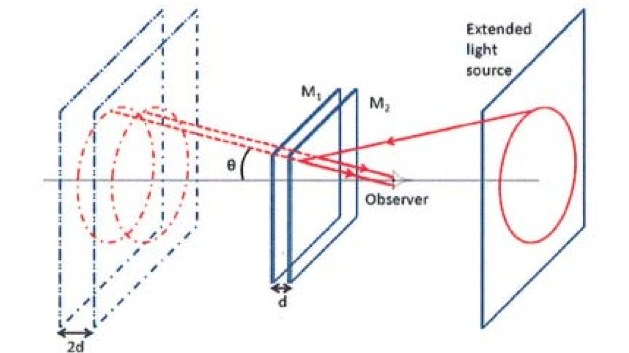
\includegraphics[height=3.5 cm, width= 6 cm]{michelson}
		\end{center}
\end{figure}

With this diagram it is easy to see that the optical path difference is given by $ OPD = 2dcos(\theta)$. When the condition described by (1.1) is met, destructive interference will occur and an observer will see a circular fringe system. 
\begin{equation}
2dcos(\theta_m) = m\lambda_0 
\end{equation}
 In this equation d is the difference in path lengths of the two arms of the interferometer, m is an integer and $\theta_m$ is the angle of the mth dark ring. So the central dark fringe will be when $\theta_m = 0$ and can be represented by $2d =m_0\lambda_0$. To measure the wavelength of the source, one can move the arms of the mirror by a distance $\Delta d$ and using the equation $\lambda =\frac{ 2 \Delta d}{N}$. \\
 \section{ Counting Fringes}
 The set-up of the lab is shown below where, the laser is aligned to both mirrors on both arms of the interferometer so that the beams that meat the target are coinciding. This insures that beam is non-dispersive throughout the experiment and the interference pattern is observed. The translational stage is connected to a microcontroller for changing the displacement of the arms.  Before the beam reaches the stage a -25 mm diverging lens into the beam to make things clearer and observe the fringe patterns better.
 \begin{figure}[htb]
	\caption{Experimental Setup}
		\begin{center}
			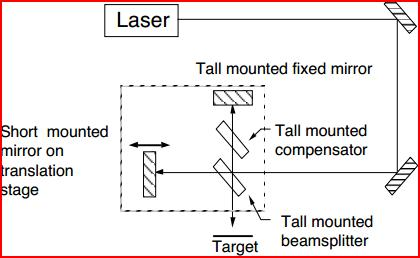
\includegraphics[scale = 0.8]{stage}
		\end{center}
\end{figure}
Once this was done, translational stage was moved and the fringes were counted, this is described by the table below.
\begin{equation}
  \begin{tabular}{| l| c | r| }
    \hline
    \lambda (nm) & N & \Delta d (m) \\ \hline
    658 & 48 & 0.0000158                     \\ \hline
    649  & 49 &    0.0000159                 \\ \hline
     615 & 53 & 0.0000163                                            \\  \hline
    644 &50 & 0.0000161                                            \\  \hline
        620 & 50 & 0.0000155                                            \\ 
    \hline
  \end{tabular}
\end{equation}

The average was 637 nm which is close to the theroretical 633 nm. 

\section{Verifying the Translational Stage Velocity}
In this part of the lab, a photodetector was replaced as the target (Fig 2.1) and connected to a oscilloscope to measure the sinusoidal pattern of the  fringes that appear on the central spot of the interfering waves, in an effort to verify the translational stage velocity. The result of sinusoidal fringe pattern is shown below,
\begin{figure}[htb]
	\caption{Intensity measurement of Central Fringe with a translational stage velocity}
		\begin{center}
			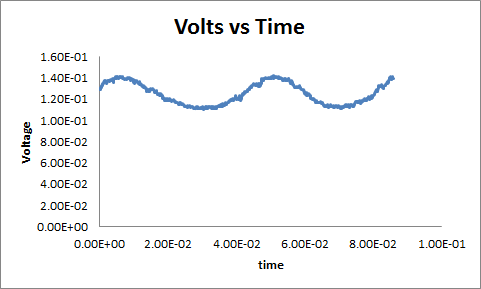
\includegraphics[scale = 0.5]{unnamed}
		\end{center}
\end{figure}

From this figure and the change in distances we find the that the stage velocity is $.07 mm/s$, the new formula for the measurment of $\lambda$ is,
\begin{equation}
\lambda  = \frac{2 v}{Nf}
\end{equation}
where $f$ is the frequency measured  of the central fringe. With this measurement 640 nm. 
\section{Precise Wavelength Measurement}
In this part of the lab we verified two different situations, the first being the Fresnel- Arago Law, which says that two orthogonal, coherent P-states cannot interfere in the sense that no fringes result. This was the case when a polarizer was placed in front of the two mirrors of the arms of the interferometer and no fringes were found. The other one being the situation  if a uncoated glass slide was placed into  one of the arms, the result was a $\pi$ phase shift because the beam has a lateral shift due to the glass but still emerges parallel to where it entered. 
%\begin{figure}[htb]
%\centering
%\parbox{5cm}{
%\includegraphics[width=5cm]{figure_1}
%\caption{ Reflection Coefficients}}
%\qquad
%\begin{minipage}{5cm}
%\includegraphics[width=5cm]{figure_2}
%\caption{Transmission Coefficients}
%\end{minipage}
%\end{figure}
%
%\begin{figure}[htb]
%\centering
%\parbox{5cm}{
%\includegraphics[width=5cm]{Epar}
%\caption{Electric Field Parallel to Incident Plane}
%\label{fig:2figsA}}
%\qquad
%\begin{minipage}{5cm}
%\includegraphics[width=5cm]{Eperp}
%\caption{Electric Field Perpendicular to Indicent Plane}
%\label{fig:2figsB}
%\end{minipage}
%%\end{figure}
%
%\section{Experiment 1.1:  Transmittance through Glass}
%\begin{figure}[!ht]
%	\caption{Experimental Set-Up}
%		\begin{center}
%			\includegraphics[scale=0.5]{transmittance}
%		\end{center}
%\end{figure}

%\begin{figure}[!ht]
%	\caption{Experimental Comparison to Theoretical Transmission Coefficients}
%		\begin{center}
%			\includegraphics[scale=0.5]{figure_3}
%		\end{center}
%\end{figure}
%
%\section{Experiment 1.2:  Reflectance from Frosted Glass}
%\begin{figure}[!ht]
%		\begin{center}
%			\includegraphics[scale=0.5]{reflectance}
%		\end{center}
%\caption{Reflectance from Frosted Glass}
%\end{figure}

%\section{Experiment 1.3: Refraction through glass slab}
%\begin{figure}[!ht]
%		\begin{center}
%			\includegraphics[scale=0.5]{GlassLab}
%		\end{center}
%\caption{Measuring the index of refraction through Glass Slab}
%\end{figure}g
% \begin{equation}
%sin(\theta_i -\theta_t) = \frac{l}{\frac{t}{cos(\theta_t)}}
% \end{equation}
% and,
% \begin{equation}
%n_{slab}  = \frac{n_1sin(\theta_1)}{sin(\theta_1-sin^{-1}(\frac{t}{\frac{l}{sin(\theta_i -\theta_t)}}))}
% \end{equation}
% Solving this $n_{slab} = 1.42$  and since most glass has a refractive index of ~1.5 this was pretty close.
 \end{document}
